\begin{enumerate}
    
    \item 
        There is no linear separator that can achieve a perfect classification score.
        
        \begin{itemize}
            \item For $0 \leq t \leq -\infty$, points $\{ (-2, 1), (2, 1) \}$ will always be misclassified as $H_{0 \leq t \leq -\infty}(x) = 1$
            \item And for $2 \leq t \leq \infty$, points $\{ (1, 1), (-1, 1) \}$ will always be misclassified as $H_{2 \leq t \leq \infty}(x) = -1$
            \item For $-2 \leq t \leq 0$, point $\{(2, 1) \}$ will always be misclassified as $H_{2 \leq t \leq 0}(x) = 1$
            \item \item For $0 \leq t \leq 2$, point $\{(-1, 1) \}$ will always be misclassified as $H_{0 \leq t \leq 2}(x) = -1$ 
        \end{itemize}
    
    \item
        $$S' = \{ (\phi(x), y): (x, y) \in S \}$$ 
        We can visually tell that the linear separation would be possible with the transformed data. The plane of maximal separation would be halfway between the two classes. That would be the line which passes through the midpoints \{(-2, 4) and (-1, 2)\} and \{(2, 4) and (1, 2)\}. 
        
        \begin{figure*}[!ht]
            \centering
            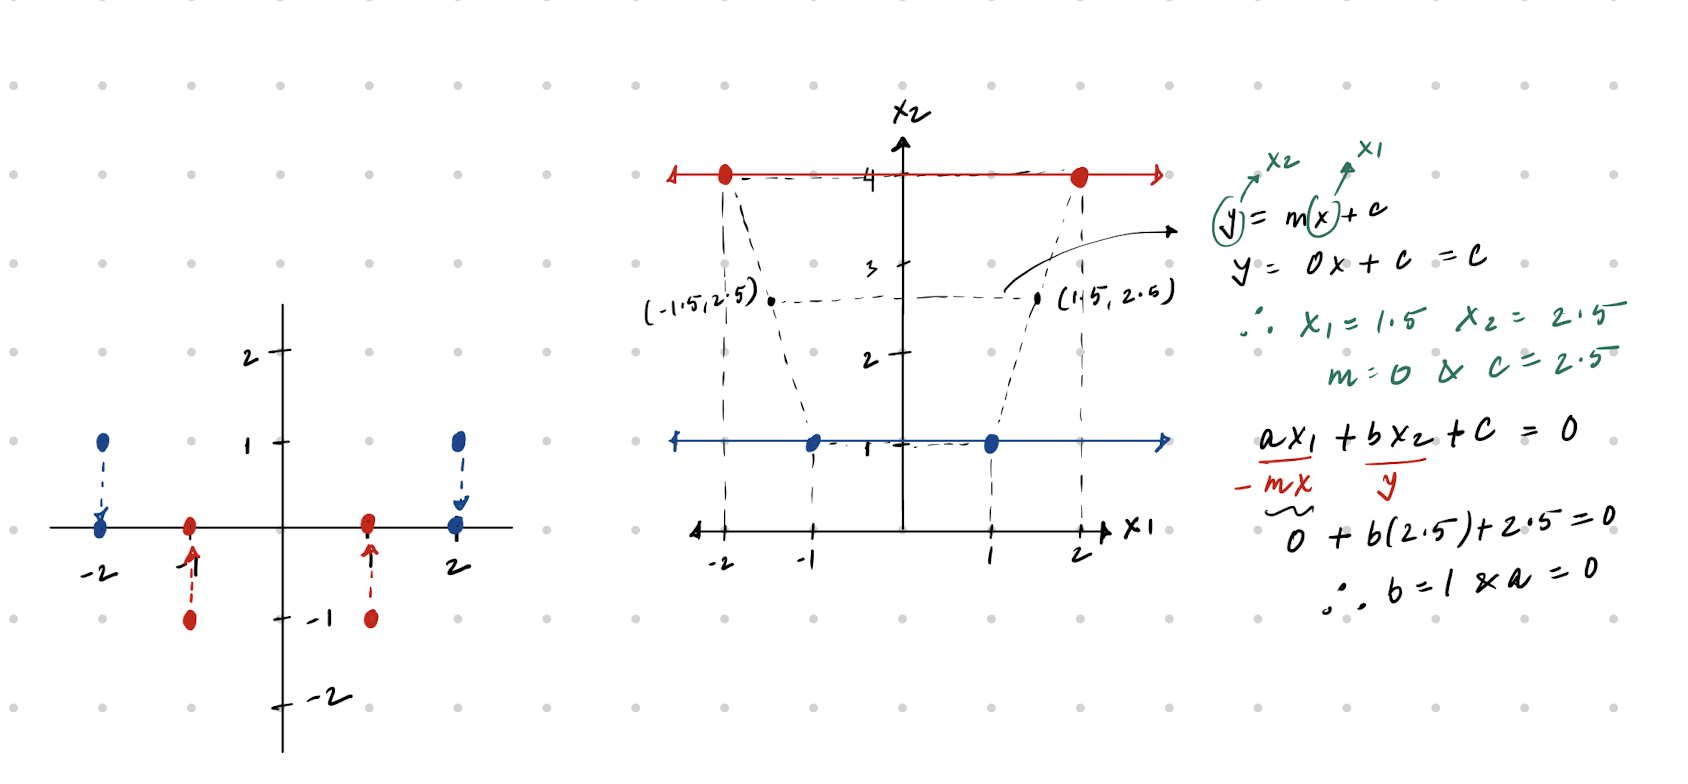
\includegraphics[width=\textwidth]{images/problem_2}
            \caption{Transformed values of $x$}
        \end{figure*}
        
        We can visually tell that the slope of the line would be zero. 
        \begin{align*}
            x_{2} & = mx_{1} + c \\
            x_{2} & = c            
        \end{align*}
        Thus we have $x_{1} = 1.5, x_{2} = 2.5, m = 0, c = 2.5$.
        \begin{align*}
            H' = \{ax_{1} + bx_{2} + c & \geq 0: a^{2} + b^{2} \neq 0 \} \\
            ax_{1} + bx_{2} + c & = 0 \\
            0 + b(2.5) + 2.5 = 0 && \text{(plugging values from above)} \\
            b = 1
        \end{align*}        
        Thus, $x_{2} \geq 2.5$ for a class to be classified as 1.
        
    \item
        Kernel function $K(x, z) = \phi(x)^{T}\phi(z) = (x, x^{2})^{T}(z, z^{2}) = xz + x^{2}z^{2}$            
        
\end{enumerate}